\section{Экспериментальное исследование}

Для экспериментальной проверки разработанного программного средства были проведены две серии экспериментов. Первая серия проведена для сравнения разработанного программного средства с наивным байесовским классификатором, используемым во многоих открытых системах фильтрации спама.

%TODO  
, а также более сложным байесовским классификатором из системы dspam. Серия призвана показать, что разработанное средство работает не хуже байесовских методов.

Вторая серия экспериментов проведена для проверки работы системы в многопрофильном режиме.

\subsection{Сравнение с наивным байесовским классификатором и байес-подобным классификатором из dspam}

\subsubsection {Набор данных}

Тестирование производилось на двух публичных наборах email-сообщений.

\begin{enumerate}
	\item SpamAssassin public corpus \cite{SAPC}
	\item CEAS 2008 Live Spam Challenge Laboratory Corpus \cite{CEAS}
\end{enumerate}

\subsubsection{Методика тестирования}

Тестирование производилось с использованием метода скользящего контроля: выборка разбивалась на пять частей, на четырех из которых проводилось обучение, а на пятой - контроль. Выборка \cite{CEAS} ввиду своей большой величины была разделена на несколько частей, на каждой из которых тестирование было произведено отдельно. 

Результат тестирования представлен в виде графика соответствия величин вероятности ложно-положительного срабатывания и вероятности верного обнаружения спама. Точка на графике обозначает что при определенной границе решающего правила система будет работать именно в таком режиме: фильтровать спам с вероятностью показанной на оси ординат и классифицировать легитимные письма как спам с вероятностью показанной на оси абцисс. Чем выше проходит график, тем более качественно работает система фильтрации.

\subsubsection{Результаты тестирования}
На графике \ref{SAPCBAYESSVM}  представлен результаты тестирования на наборах \cite{SAPC}. Видно, что разработанное средство всегда работает лучше чем наивный байесовский классфикатор.

Байесовский классификтор из системы dspam показывает примерно такие же результаты, что и разработанный метод.
\begin{figure}[h]
\begin{center}
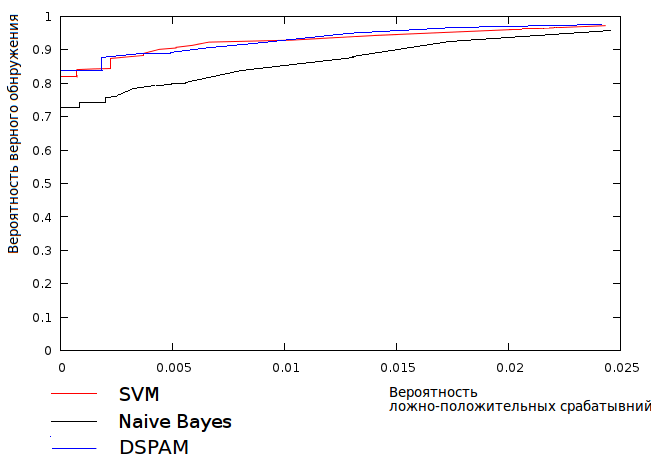
\includegraphics[width=15cm]{img/graphic}
\end{center}
\caption{Сравнение качества тестирования реализованного алгоритма, наивного байесовского классификатора на наборе\cite{SAPC}}
\label{SAPCBAYESSVM}
\end{figure}

Тестирование на наборе \cite{CEAS} дало аналогичный же результат.

\subsection{Тестирование работы в многопрофильном режиме}

\subsubsection{Набор данных}
Тестирование производилось на наборе данных SpamAssassin Public Corpus \cite{SAPC}.
Для проведения эксперимента сообщения, представленные в выборке были разделены на 3 класса:
\begin{enumerate}
\item Класс, сообщения из которого все письма считаются легитимной почтой.
\item Класс, сообщения из которого все пользователи считают спамом
\item Класс, сообщения из которого считают спамом некоторые из пользователей
\end{enumerate}

В класс 1 были включены все сообщения, отмеченные в наборе \cite{SAPC} как спам. Классы 2 и 3 были получены из писем, отмеченных в наборе \cite{SAPC} как легитимная почта.
\begin{enumerate}
	\item Эксперимент показывающий, что новые добавление пользователей не ухудшает качество фильтрации.

	Для проведения эксперимента использовались классы писем 1 и 2. Каждый из классов был поделен случайным образом на две части. Эти части считались обучающими выборками для двух разных пользователей. Далее было произведена проверка метода при помощи скользящего контроля, с учетом того, что в системе теперь не один а два пользователя.

	\item Эксперимент показывающий что многопрофильность работает, и обучение на данных одного пользователя распространяется на другого. Сообщения из всех трех классов были разделены на две части(для первого и второго пользователей). Обучение производилось на всех трех наборах для первого пользователя и на первых двух для второго. Далее было произведено тестирование второго пользователя на сообщениях из третьей группы и посчитаны оценкивероятности принадлежности к спаму для писем. На результируещем графике показаны диапазоны вероятности и количество писем попавших в этот диапазон.

	\item Эксперимент показывающий что разное мнение пользователей о группе писем не приводит к проблемам. Эксперимент аналогичен предыдущему, за исключением того, что второй пользователь также обучался на письмах из третьей группы. На результирующем графике представлены диапазоны вероятности и количество писем попавших в этот диапазон для первого и второго пользователей. 
	
\end{enumerate}
\subsubsection{Результаты}
На графиках представлены результаты тестирования работы средства в многопрофильном режиме. 

Из графика \ref{EXPERIMENT2} видно, что обучение на одном пользователе распространяется на другого пользователя.

Из графика \ref{EXPERIMENT3} видно, что если мнения пользователей о каком-то классе писем различны, то система так же будет работать корректно.
\begin{figure}[h]
\begin{center}
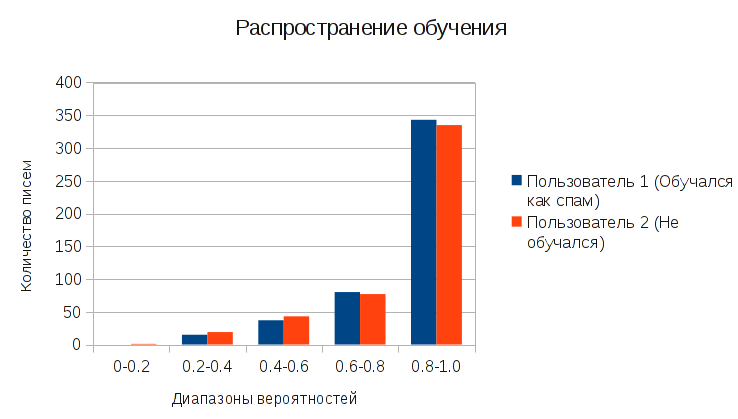
\includegraphics[width=15cm]{img/experiment2}
\end{center}
\caption{Результаты тестирования пользователя на третьем тестовом наборе. Обучение было произведено на другом пользователе \cite{SAPC}}
\label{EXPERIMENT2}
\end{figure}

\begin{figure}[h]
\begin{center}
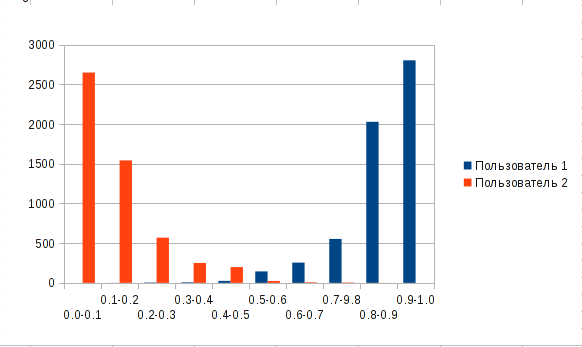
\includegraphics[width=15cm]{img/experiment3}
\end{center}
\caption{Результаты тестирования на третьем тестовом наборе после обучения на данных из этого набора для каждого из пользователей. Видно что у одного пользователя письма из этого набора определяются как спам, а у другого как легитимная почта.}
\label{EXPERIMENT3}
\end{figure}

